\sectionmark{Regulation}

\section{Regulation}
\begin{enumerate}
	\item In der Glykolyse sind die Phosphofructokinase und die Pyruvatkinase Angriffsorte der allosterischen Regulation. Warum ist das sinnvoll?

		Die Funktion der Phosphfructokinase (PfK) wird positiv beeinflusst von ADP.
		und negativ vom Vorhandensein von Phosphoenolpyruvat (PEP).	
		Gleichzeitig hat das Fructose-1,6-bis-Phosphat einen positiven Einfluss auf die Expression
		der Pyruvatkinase.

		Letzlich sorgen diese Regulation dafür,
		das wenn ATP verbraucht wird und somit ein große Menge ADP zuv Verfügung steht,
		dass Pyruvat gebildet wird.
		Gleichzeit sorgen die positiven und negativen Einflüße dafür,
		das dies Effizient geschieht und keine Proteine gebildet werden,
		die nicht benötigt werden.
		Sie hierzu Folien zur Vorlesung Regulation, Seite 7 unten. 
		%TODO hier nen schickes bild dazu einbauen.

	\item Warum ist es so wichtig, dass Mikroorganismen sehr schnell auf äußere Einflüsse reagieren können? Können Sie sich Bakterien vorstellen, die weitgehend ohne regulatorische Vorgänge auskommen können?

		Da Mikoorganismen ihr Habitat kaum wechseln können müssen sie in der Lage sein,
		sich Veränderung möglichst schnell anzupassen.

		Mikroorganismen in Symbiotischen Beziehungen können (wahrscheinlich) auf Regulationen verzichten,
		welche zur Regulation der Substrat aufnahme dienen.
		Sollten diese sich ändern werden sie durch ihre Bindung an den Symbionten kaum in der Lage sein,
		eine Veränderung zuertragen.

	\item Wie kann die Aktivität von Proteinen, z.B. von Enzymen oder Regulatoren moduliert werden? Nennen Sie für wenigstens zwei der Mechanismen Beispiele!

		\begin{description}
			\item[Substrat] \hfill \\
				Das vorhandene Substrat die Aktivität von Enzymen modulieren.
				Als Beispiel kann hier das \slshape{lac}-Operon dienen.
				Dieses sorgt dafür das von \emph{E. coli} zunächst nur Glucose verwertet,
				selbst wenn auch Lactose zur Verfügung steht.
				Diese wird erst verstoffwechselt,
				wenn keine Glucose mehr zur Verfügung steht.
			\item[Induktoren] \hfill \\
				Bestimmte Proteine können für die explizite Exprimierung von Genen dienen. % orly?
			\item[micro-RNAs] \hfill \\
				kleine RNA-Abschnitte können mit der mRNA binden und ihre Translation verhindern.
		\end{description}

	\item Wodurch zeichnen sich gute Promotoren aus? Tatsächlich sind nur wenige Promotoren wirklich gut! Warum ist es für die Organismen vorteilhaft, suboptimale Promotoren zu besitzen? 

		Wenn Promotoren nicht die optimale, komplementäre Sequenz haben an die die RNA-Polymerase bindet,
		reduziert sich die Wahrscheinlichkeit das das Protein erzeug wird.
		So lässt sich modulieren,
		das weniger von diesem Protein benötigt wird.

	\item Erläutern Sie den Aufbau der RNA-Polymerase?	

		Die RNA-Polymerase besteht aus 5 Untereinheiten.
		Das sind:
		\begin{itemize}
			\item 2 \begin{math}\alpha\end{math}-Untereinheiten
			\item \begin{math}\beta\end{math}-Untereinheiten
			\item \begin{math}\beta\end{math}'-Untereinheiten
			\item \begin{math}\sigma\end{math}-Untereinheiten
		\end{itemize}

	\item Unter welchen Bedingungen wird das lac-Operon von \emph{E. coli} exprimiert? Stellen Sie sich vor, Sie hätten eine Mutante, in der das Gen für die Lac-Permease zerstört ist. Wie wird das lac-Operon in dieser Mutante exprimiert, wenn Lactose in Medium vorhanden ist?
	
		Die ß-Galaktosidase, zur Umsetzung von  Lactose,
		wird nur gebildet wenn Glucose im Medium aufgebraucht ist und 
		Lactose im Medium vorhanden ist.
		
		An der Regulation sollte sich nichts ändern,
		jedoch wird die Lactose nicht bis ins Zellinnere kommen,
		da dafür die Lac-Permease verantwortlich ist.
		
	\item \emph{Bacillus subtilis} kann keine Lactose verwerten, dafür aber Fruktose. Was vermuten Sie, unter welchen Bedingungen werden die Gene für die Fruktoseverwertung exprimiert und unter welchen nicht?	

		Die Regulation sollte ähnlich wie beim lac-Operon erfolgen,
		da Fruktose ähnlich wie Lactose nur schwerer zu verwerten ist.

	\item Gene für die Fruktoseverwertung kodieren für eine PTS-Fruktosepermease und für ein Enzym, das Fruktose-1,6-Bisphosphat bildet. Wie sieht dann der weitere Stoffwechsel aus? Die Aktivität welcher Enzyme dieses Stoffwechselweges wird durch Metaboliten reguliert?

		(Es findet letzlich ein Umwandlug in Pyruvat statt.
		Die Steuerung erfolgt über das Vorhandensein von Glucose im Medium.)
		%TODO verifizieren

	\item Erklären Sie die Rolle der Adenylatzyklase, des Lac-Repressors und des Crp-Proteins für die Expression des lac-Operons.

		\begin{description}
			\item[Adenylatzyklase] \hfill \\
				Die Adenylatzyklase ist verantwortlich für die Bildung des Signalmoleküls cAMP,
				welches der Kofaktor des Crp-Proteins ist.
				Crp wird von cAMP aktiviert.
			\item[Lac-Repressor] \hfill \\
				Der Lac-Repressor reprimiert die Expression des Lac-Operons,
				und verhindert den Abbau von Lactose.
				Ist Crp aktiv, wird der Lac-Repressor gebunden
				und Lactose kann abgebaut werden.
			\item[Crp-Protein] \hfill 
				Das Crp-Protein kann nur durch cAMP aktiviert werden 
				und bindet wenn es aktiviert ist den Lac-Repressor,
				damit Lactose abgebaut werden kann.
		\end{description}

	\item Ein Schlüsselfaktor bei der Katabolitenrepression in \emph{E. coli} ist das Crr Protein. Erklären Sie die duale Funktion dieses Proteins!	
	\item Wie sind Zweikomponentensysteme aufgebaut und wie werden die Signale in ihnen weitergeleitet?

		Bei Zweikomponentensystemen ist die Signalerkennung und die Signalweitergabe auf zwei Proteine verteilt.
		Hierbei ist die Signalerkennung meist membranständig und die Signalweitergabe ist meist eine DNA-bindeendes Protein
		bzw. das Substrat des Proteins zur Signalerkennung.

	\item Was verstehen Sie unter einem RNA-Schalter, was unter einem Riboswitch?

		Ein Riboswitch ist ein Teil einer mRNA der direkt mit einem niedermolekularen Metaboliten binden kann
		und so die Genregualation moduliert.
		Dabei können sie auch die Transkription und Translation der eigenen mRNA regulieren.
		%Gibt es wirklich einen unterschied?!

	\item Die Transkription der trp-Operons in \emph{E. coli} und \emph{B. subtilis} wird frühzeitig abgebrochen, wenn Tryptophan im Medium vorhanden ist. Erklären Sie anhand einer Skizze, wie diese Regulation zustande kommt und diskutieren Sie Gemeinsamkeiten und Unterschiede der Regulationsmechanismen in den beiden Bakterien!

		Siehe Folien zur Vorlesung Regulation S.26.

		Die Regulation in \emph{E. coli} geschieht durch eine Leader-Protein.
		Dieses enthält Tryptophan und wird somit nur fertig translatiert,
		wenn Tryptophan vorhanden ist.
		Die mRNA, auf dem dieses Leader Protein liegt,
		kann nach der Translation des Leader bereichs aber nicht Fortschreiten,
		da sich ein Riboswitch aus der ``Attenuator''-Struktur gebildet hat.
		Dieses verhinder die weiter Synthese von Proteinen zu Trypthophansynthese (da ja Tryptophan vorhanden ist).

		Kann die Leadersequenz auf Grund von wenig oder keinem Tryptophan nur langsam,
		oder garnicht translatiert werden.
		Die ``Attenuator''-Struktur formt eine andere Struktur,
		die die weiter Translation von Tryptophan-synthetisierden Proteinen erlaubt.
		
		\begin{figure}[ht!]
		\leavevmode
		\begin{center}
		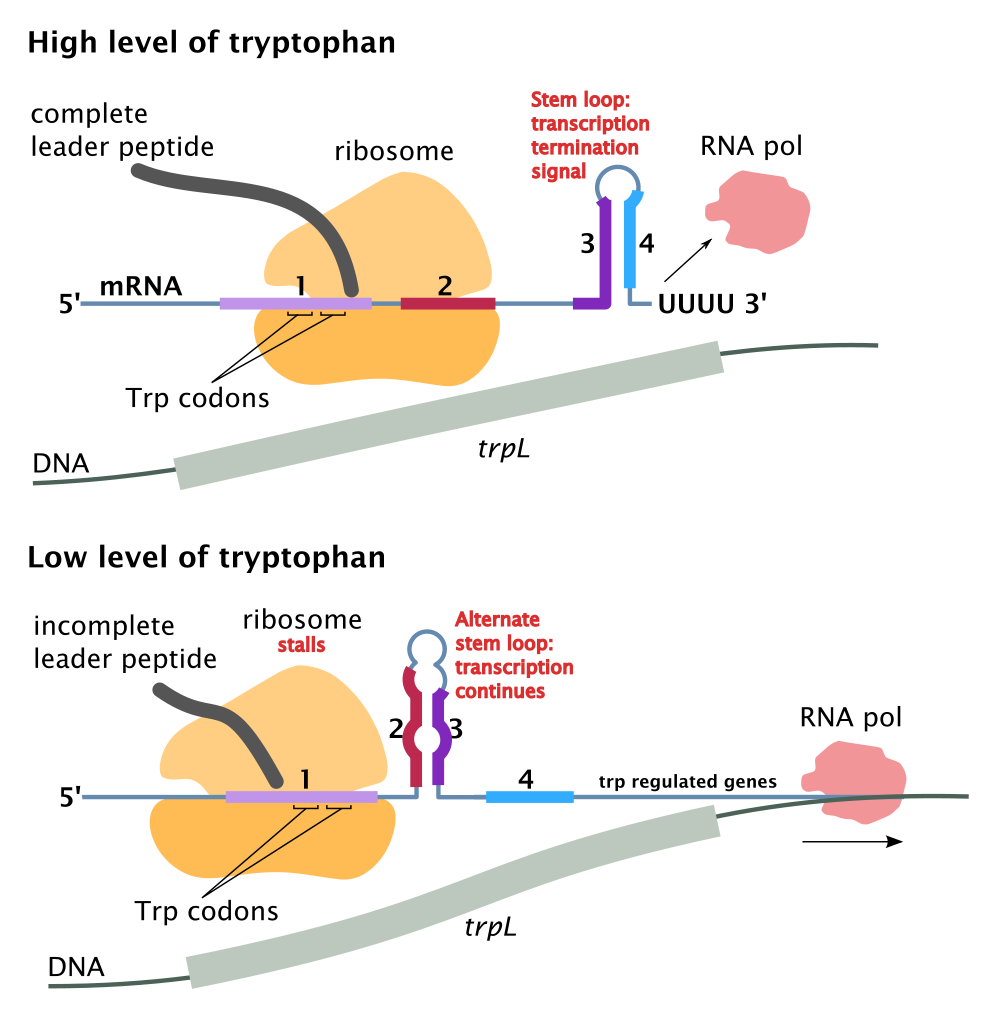
\includegraphics[scale=0.32]{./pictures/trp_operon_1000}
		\end{center}
		\caption{\slshape{Trypthophan Operon in \emph{E. coli}.}}
		\label{fig:trpoperon}
		% http://en.wikipedia.org/wiki/File:Trp_operon_attenuation.svg
		\end{figure}

\end{enumerate}
